\section{Performance Evaluation}
    \subsection*{Training ANN}
        
        An ANN with structure $[784-20-10]$ with sigmoid activation function is constructed and compiled with stochastic gradient descent (SGD) as optimizer and mean square error (MSE) as loss function. The network consists of one hidden layer with $20$ neurons and one output layer with $10$ neurons. 

        The compiled network is trained on a subset of MNIST dataset consisting of random $600$ training samples and $100$ testing samples. The network was able to achieve training accuracy of $96\%$ and testing accuracy of $89\%$. \Cref{fig:training_results} illustrates testing performance of trained network.

        \begin{figure}[htbp]
            \centering
            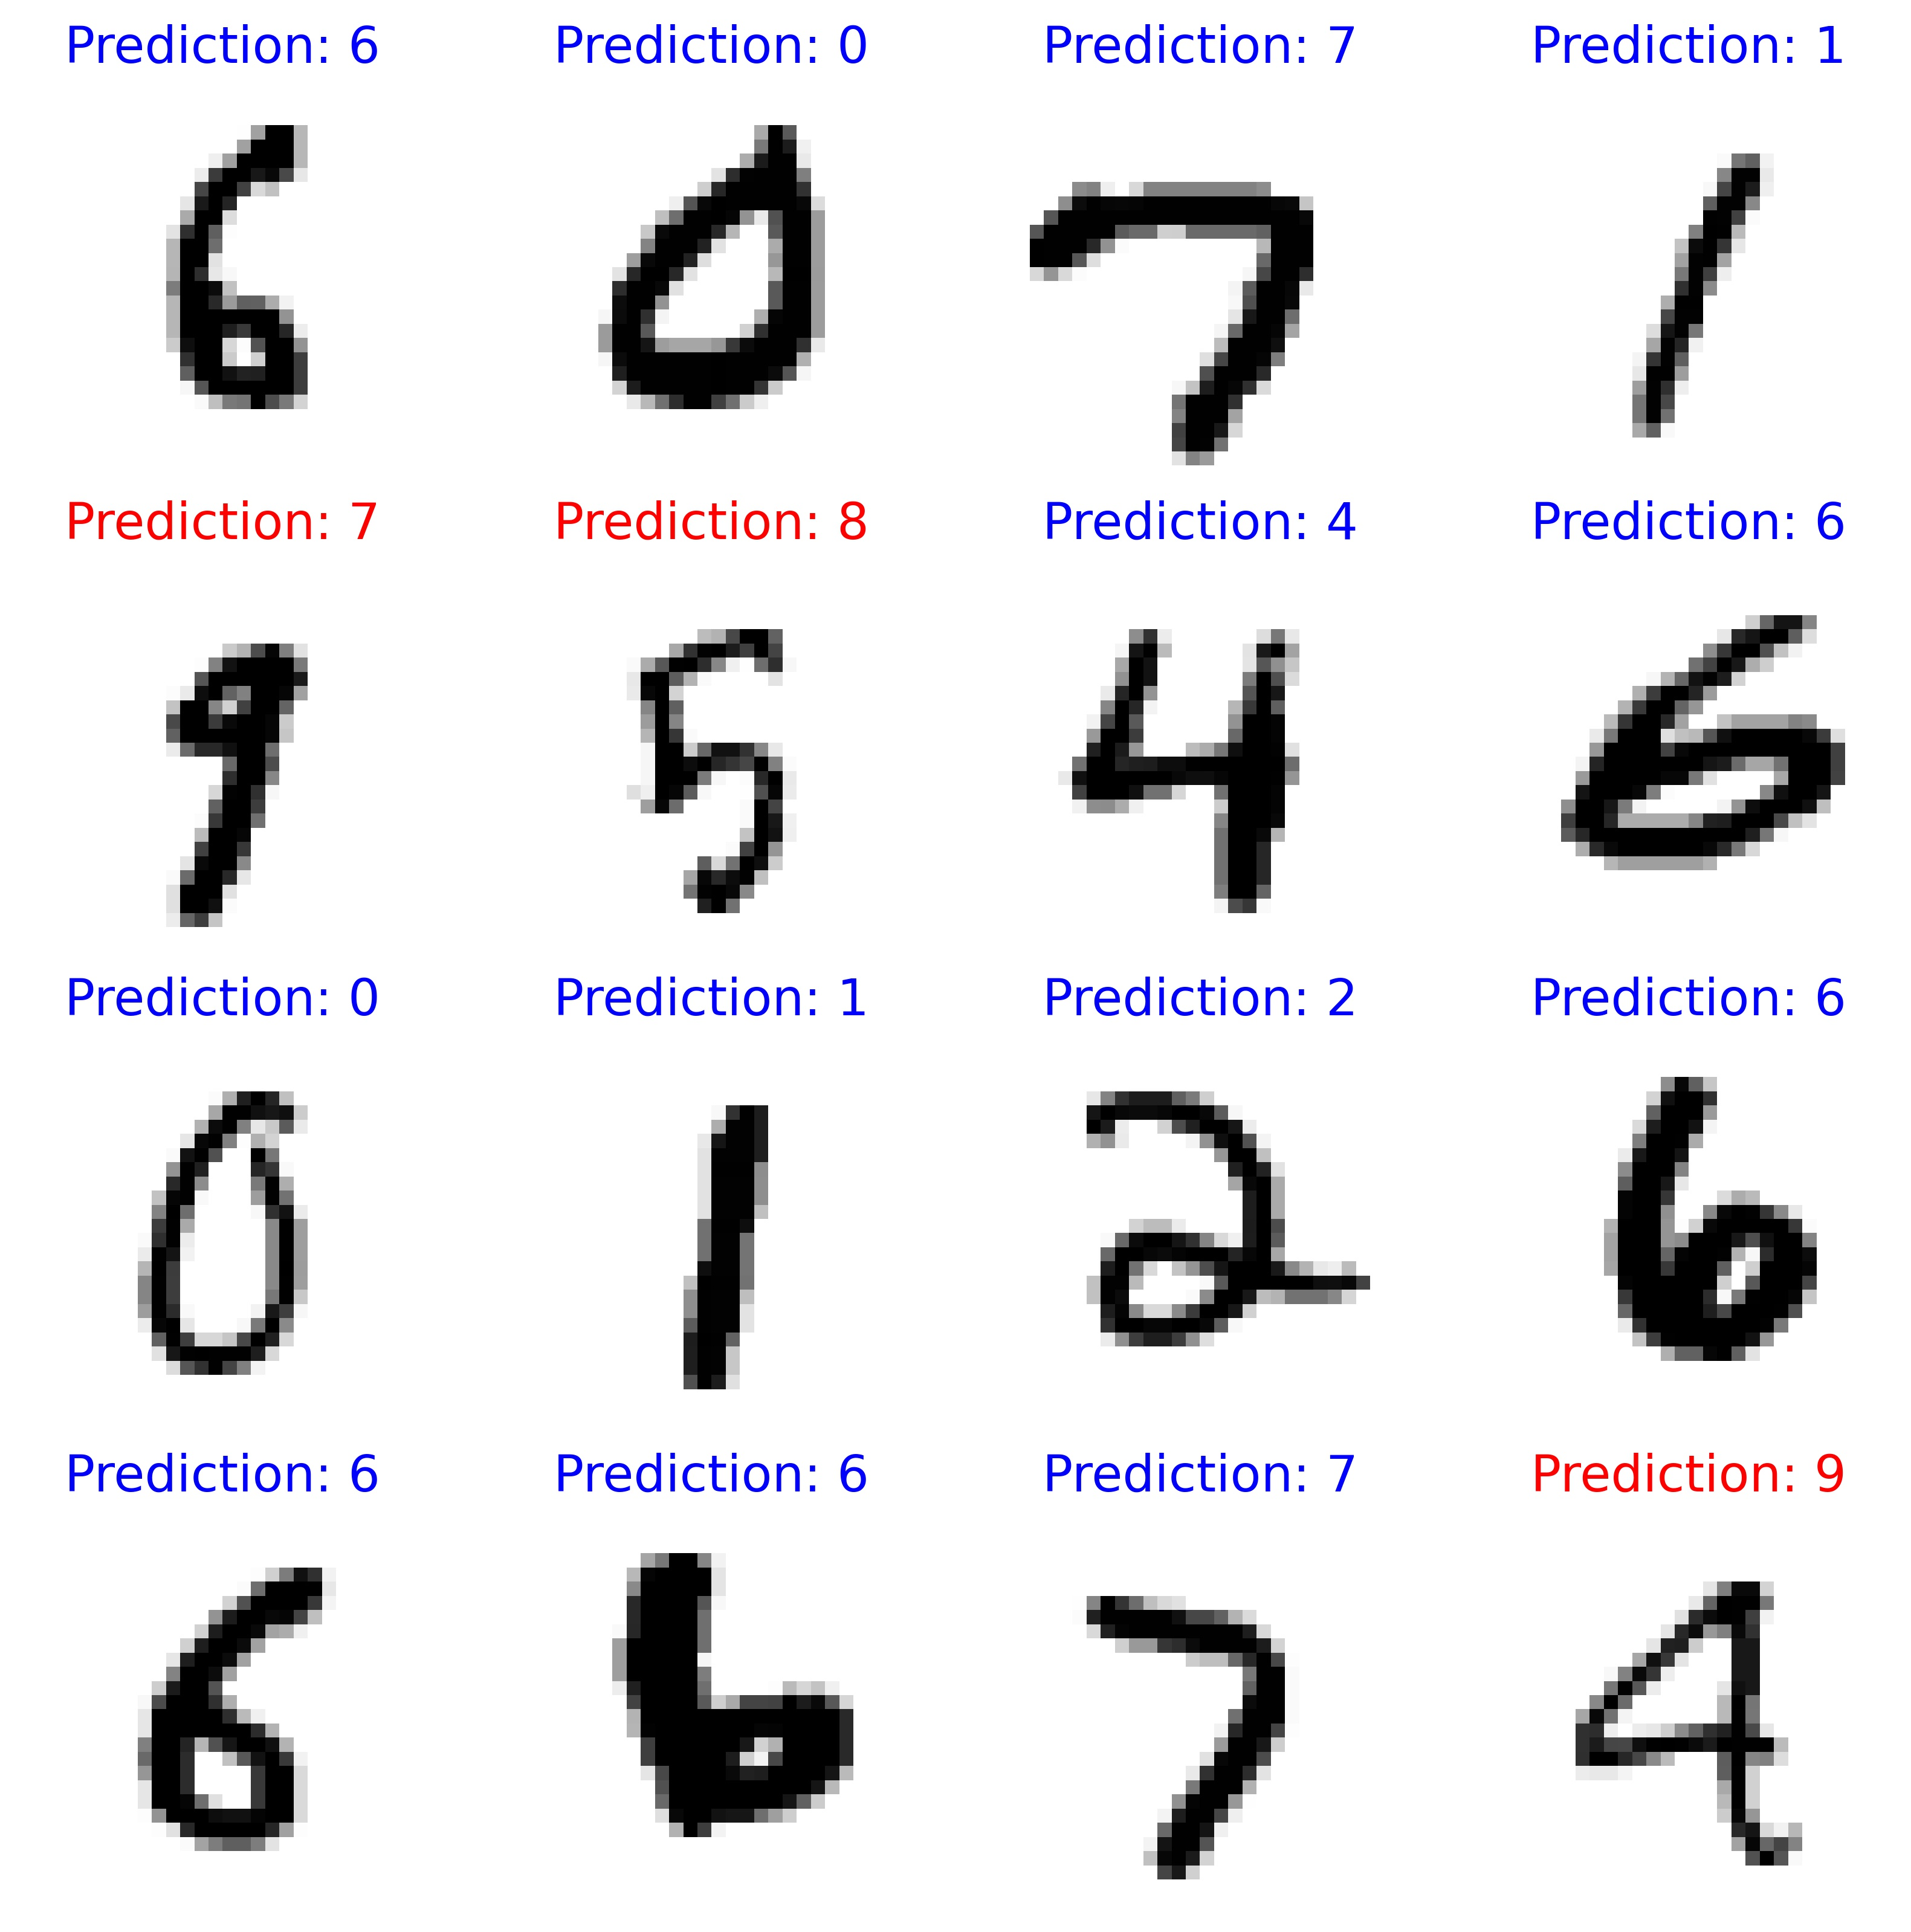
\includegraphics[width=\linewidth]{images/trained_predictions.jpg}
            \caption{Predictions of trained network on test set}
            \label{fig:training_results}
        \end{figure}

    \subsection*{Target Adversarial Attack}

        For generating adversarial images, \crefrange{alg:generate_image}{alg:update_weights} are used where  adversary just need to pass target image $(x^{Adv})$ and goal $(Y^{Adv})$ in \cref{alg:generate_image}. For generating adversarial images $\lambda = 0.8$ is considered. A noise will be generated as an adversarial image if $\lambda = 0$ is considered. \Cref{fig:adversarial_images} consists of all generated adversarial images using which target adversarial attack was successful. Some generated images as shown in \cref{fig:adversarial_images_unsuccessful} were not able to fool the trained network, but it is worth to notice that network confidence in correctly predicting particular image is decreased. 

        \begin{figure}[htbp]
            \centering
            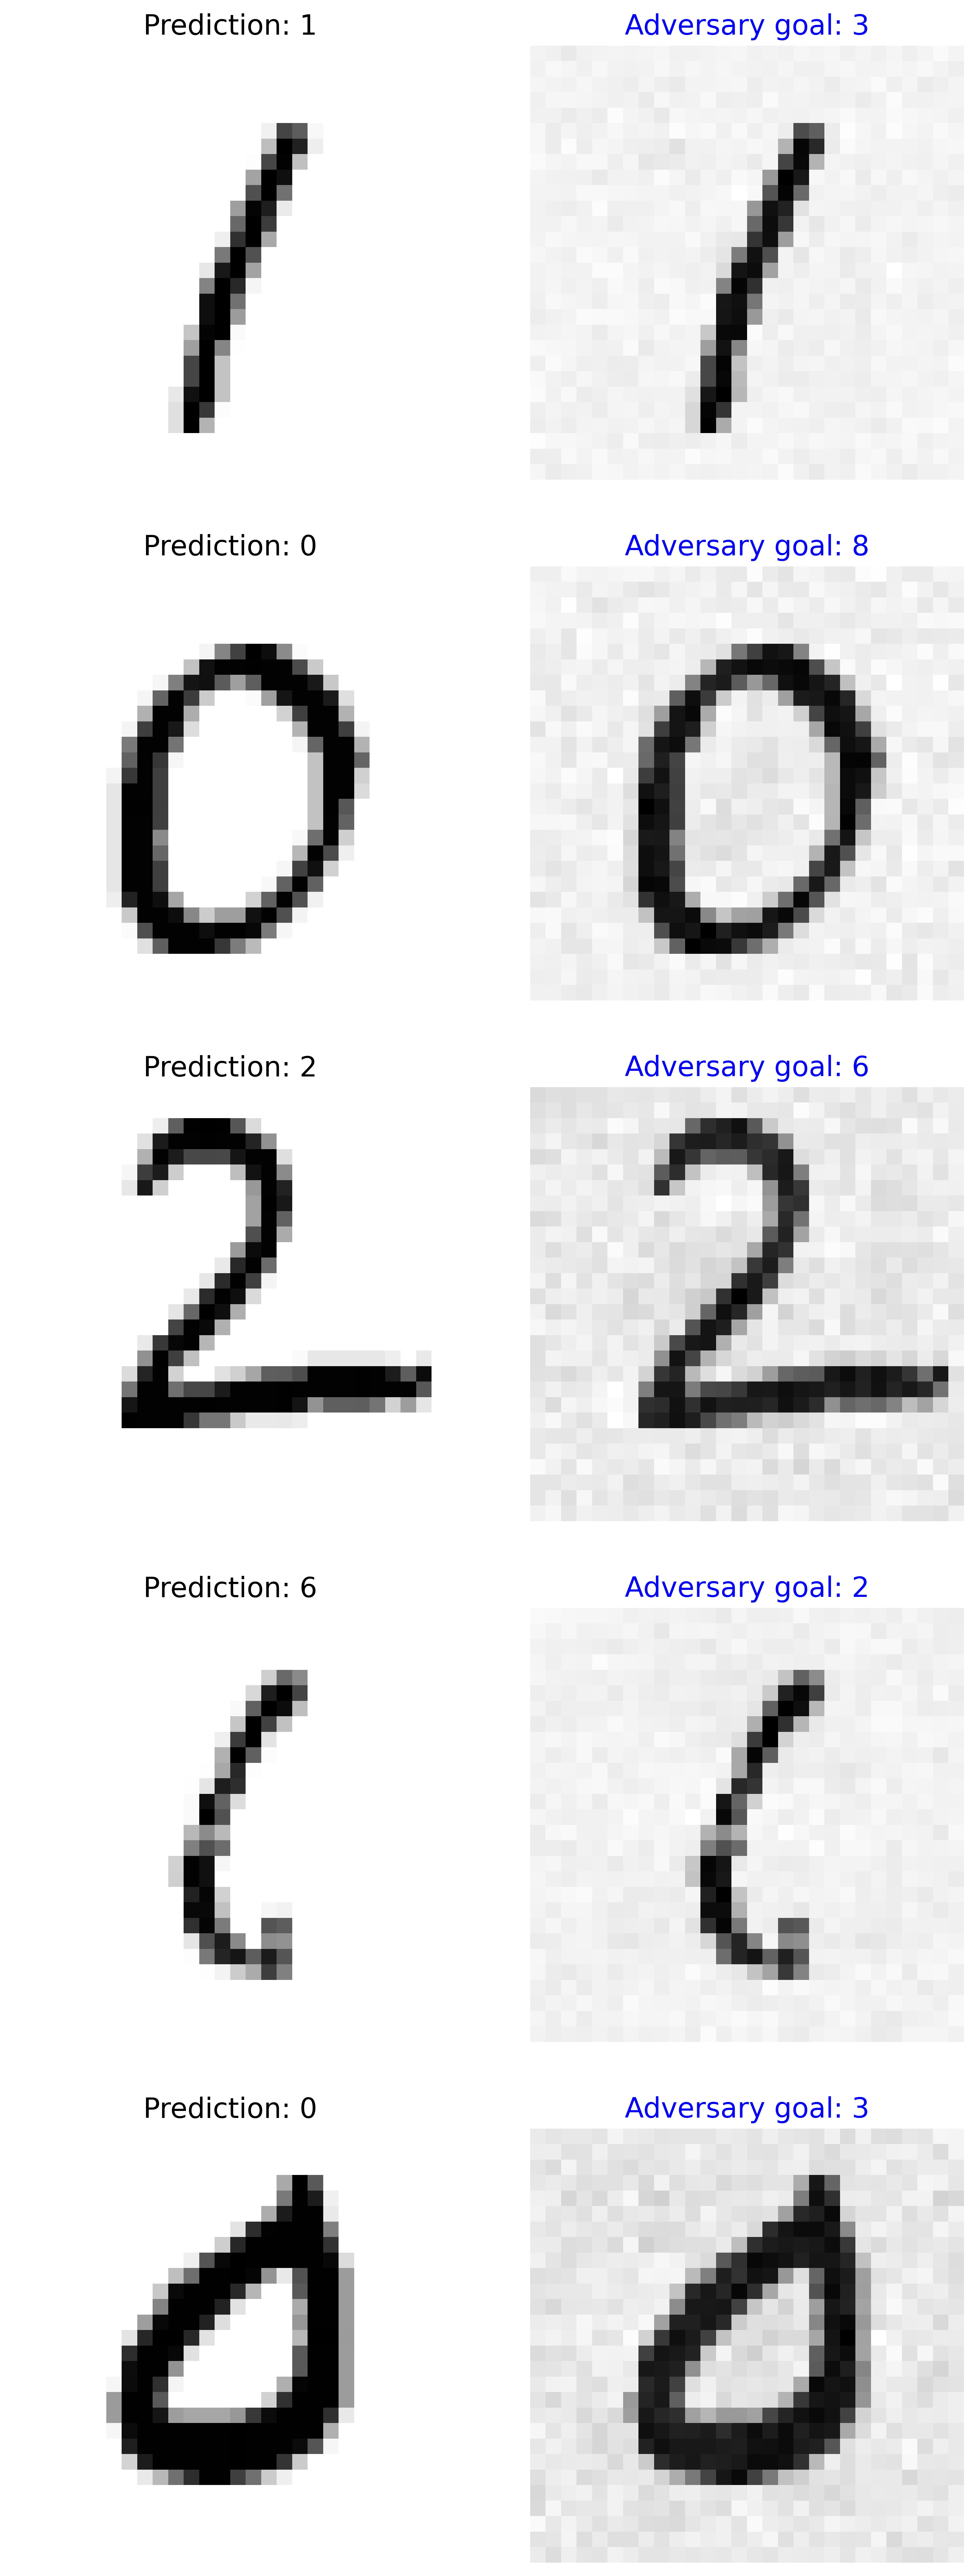
\includegraphics[width=\linewidth]{images/generated_adversarial_images.jpg}
            \caption{Some target adversarial images (in left) and generated adversarial images (in right) with adversary goal and actual prediction}
            \label{fig:adversarial_images}
        \end{figure}

        \begin{figure}[htbp]
            \centering
            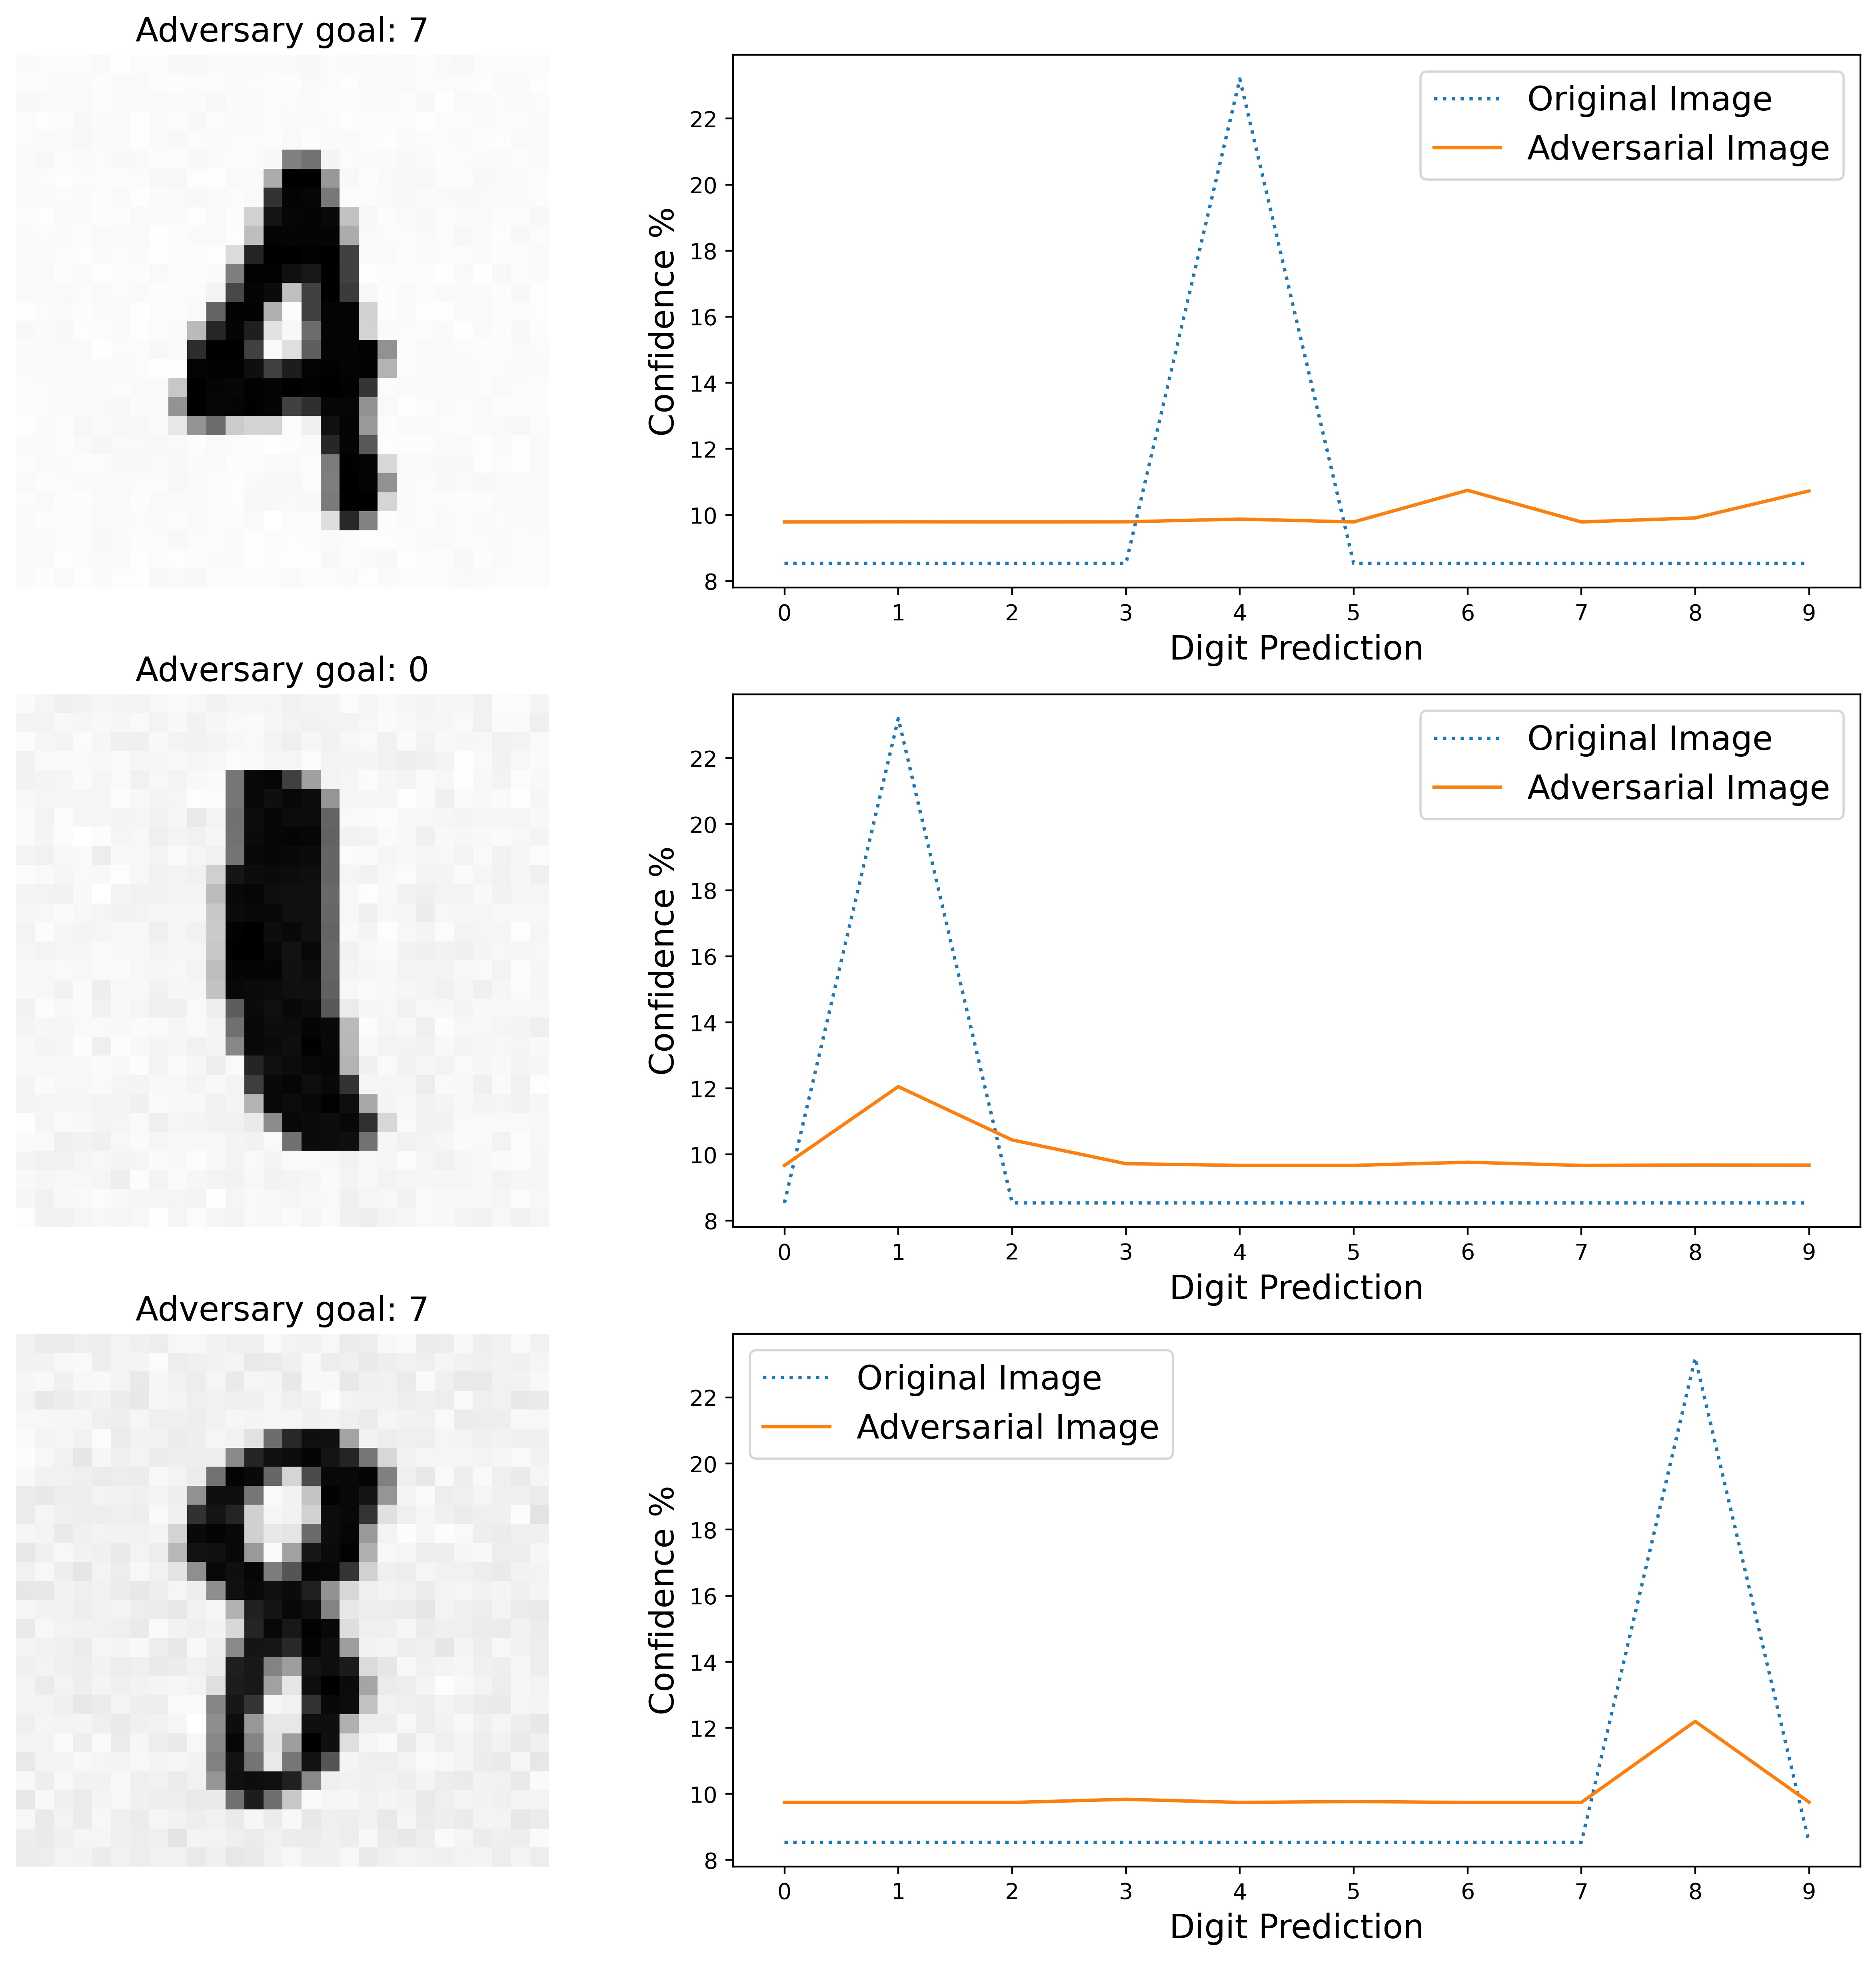
\includegraphics[width=\linewidth]{images/generated_adversarial_images_unsuccessful.jpg}
            \caption{Some target adversarial images (in left) and generated adversarial images (in right) with adversary goal and actual prediction}
            \label{fig:adversarial_images_unsuccessful}
        \end{figure}

    